%=====================================================================
%  HEMPCRETE IS A SUSTAINABLE MATERIAL — Seminar Report
%  Aryan O S, SNM23CE003, Dept. of Civil Engineering, SNMIMT Maliankara
%  Formatted to match the department sample report (Reference.pdf):
%  12 pt Times New Roman, 1.5 line spacing, 3.5 cm / 2 cm margins,
%  page number centred at the foot, no running header.
%  COMPILE WITH XeLaTeX (fontspec / Times New Roman).
%=====================================================================
\documentclass[12pt,a4paper,final]{report}

\usepackage[left=3.5cm,right=2cm,top=2.51cm,bottom=2.91cm,footskip=1.08cm]{geometry}
\usepackage{fontspec}
\setmainfont{Times New Roman}

\usepackage{graphicx}
\usepackage{setspace}
\usepackage{ragged2e}
\usepackage{array}
\usepackage{booktabs}
\usepackage{tabularx}
\usepackage{longtable}
\usepackage{float}
\usepackage{caption}
\usepackage{enumitem}
\usepackage{etoolbox}
\usepackage{titlesec}
\usepackage{tocloft}
\usepackage{fancyhdr}
\usepackage[hidelinks]{hyperref}

\linespread{1.4276}  % 20.7 pt baselines, matching the sample report
\justifying
\setlength{\parindent}{0pt}
\setlength{\parskip}{0pt}

% ---------- page style: number centred at the foot, no header ----------
\pagestyle{fancy}
\fancyhf{}
\fancyfoot[C]{\thepage}
\renewcommand{\headrulewidth}{0pt}
\renewcommand{\footrulewidth}{0pt}
\fancypagestyle{plain}{\fancyhf{}\fancyfoot[C]{\thepage}%
  \renewcommand{\headrulewidth}{0pt}\renewcommand{\footrulewidth}{0pt}}

% ---------- chapter and section headings ----------
% CHAPTER n  (16 pt bold, centred) over the chapter title (16 pt bold, centred)
\titleformat{\chapter}[display]
  {\centering\bfseries\fontsize{16}{20}\selectfont}
  {CHAPTER \thechapter}{-0.7pt}{\fontsize{16}{20}\selectfont}
\titlespacing*{\chapter}{0pt}{-8pt}{10.5pt}
\titleformat{\section}{\bfseries\fontsize{14}{18}\selectfont\raggedright\hyphenpenalty=10000\exhyphenpenalty=10000}{\thesection}{0.6em}{}
\titlespacing*{\section}{0pt}{17.6pt}{1.7pt}
\titleformat{\subsection}{\bfseries\fontsize{12}{16}\selectfont\raggedright\hyphenpenalty=10000\exhyphenpenalty=10000}{\thesubsection}{0.6em}{}
\titlespacing*{\subsection}{0pt}{17.6pt}{1.7pt}

% unnumbered front-matter headings, same look as a chapter title
% front-matter heading: 16 pt bold, ~45 pt below the top line, ~42 pt gap after
\newcommand{\frontheading}[1]{%
  \vspace*{4.1pt}%
  \begin{center}{\bfseries\fontsize{16}{16}\selectfont #1}\end{center}%
  \vspace{0.6pt}}

% ---------- figure captions: "Fig 3.1 Caption", centred, 12 pt ----------
\captionsetup[figure]{labelfont={bf},labelsep=space,name=Fig,
                      justification=centering,font=small,skip=6pt}
\captionsetup[table]{labelfont={bf},labelsep=space,
                     justification=centering,font=small,skip=6pt}
\renewcommand{\thefigure}{\thechapter.\arabic{figure}}

% ---------- Contents / List of Figures in the sample report's style ----
\renewcommand{\cfttoctitlefont}{\hfill\bfseries\fontsize{16}{20}\selectfont}
\renewcommand{\cftaftertoctitle}{\hfill}
\renewcommand{\cftloftitlefont}{\hfill\bfseries\fontsize{16}{20}\selectfont}
\renewcommand{\cftafterloftitle}{\hfill}
\renewcommand{\contentsname}{CONTENTS}
\renewcommand{\listfigurename}{LIST OF FIGURES}
\setlength{\cftbeforechapskip}{0pt}
\setlength{\cftbeforesecskip}{0pt}
\renewcommand{\cftchapfont}{\normalfont\hyphenpenalty=10000\exhyphenpenalty=10000}
\renewcommand{\cftchappagefont}{\normalfont}
\renewcommand{\cftchapleader}{\cftdotfill{\cftnodots}}
\renewcommand{\cftchappresnum}{CHAPTER~}
\renewcommand{\cftchapaftersnum}{}
\setlength{\cftchapnumwidth}{2.5cm}
\renewcommand{\cftfigpresnum}{}
\renewcommand{\cftfigaftersnum}{}
\renewcommand{\cftsecfont}{\normalfont\hyphenpenalty=10000\exhyphenpenalty=10000}
\setlength{\cftsecindent}{1.2cm}
\setlength{\cftfigindent}{0pt}
\setlength{\cftfignumwidth}{1.8cm}
\renewcommand{\cftfigfont}{\normalfont\hyphenpenalty=10000\exhyphenpenalty=10000}
\renewcommand{\cftsecleader}{\cftdotfill{\cftnodots}}
\renewcommand{\cftfigleader}{\cftdotfill{\cftnodots}}

\begin{document}
\sloppy

%=====================================================================
% TITLE PAGE
%=====================================================================
\pagenumbering{gobble}
\thispagestyle{empty}
\begin{center}
\linespread{1}\selectfont
\setlength{\parskip}{0pt}
\vspace*{-3.5pt}
{\bfseries\fontsize{16}{19.2}\selectfont HEMPCRETE IS A SUSTAINABLE MATERIAL}\\[16.3pt]
{\bfseries\fontsize{12}{14.4}\selectfont SEMINAR REPORT}\\[11.4pt]
{\fontsize{12}{14.4}\selectfont Submitted by}\\[38.8pt]
{\bfseries\fontsize{14}{16.8}\selectfont ARYAN O S}\\[14.0pt]
{\bfseries\fontsize{12}{14.4}\selectfont SNM23CE003}\\[13.2pt]
{\fontsize{12}{14.4}\selectfont To}\\[24.7pt]
{\fontsize{12}{14.4}\selectfont The APJ Abdul Kalam Technological University}\\[22.1pt]
{\fontsize{12}{14.4}\selectfont In partial fulfillment of the requirements for the award of the Degree of}\\[11.3pt]
{\fontsize{12}{14.4}\selectfont Bachelor of Technology In}\\[11.4pt]
{\itshape\fontsize{12}{14.4}\selectfont Civil Engineering}\\[26pt]

\includegraphics[height=3.8cm]{snmlogo.png}\\[27.7pt]
{\bfseries\fontsize{14}{16.8}\selectfont Department of Civil Engineering}\\[32.4pt]
{\bfseries\fontsize{14}{16.8}\selectfont SREE NARAYANA MANGALAM INSTITUTE OF MANAGEMENT}\\[19.9pt]
{\bfseries\fontsize{14}{16.8}\selectfont \& TECHNOLOGY}\\[33.5pt]
{\bfseries\fontsize{14}{16.8}\selectfont MALIANKARA}\\[40.3pt]
{\fontsize{14}{16.8}\selectfont SEPTEMBER, 2026}
\end{center}

%=====================================================================
% CERTIFICATE
%=====================================================================
\newpage
\thispagestyle{empty}
\begin{center}
\linespread{1}\selectfont
\setlength{\parskip}{0pt}
\vspace*{20.4pt}
{\bfseries\fontsize{14}{16.8}\selectfont DEPARTMENT OF CIVIL ENGINEERING}\\[45.7pt]
{\bfseries\fontsize{14}{16.8}\selectfont SREE NARAYANA MANGALAM INSTITUTE OF MANAGEMENT}\\[4.1pt]
{\bfseries\fontsize{14}{16.8}\selectfont \& TECHNOLOGY, MALIANKARA}\\[32.6pt]

\includegraphics[height=3.8cm]{snmlogo.png}\\[27.7pt]
{\bfseries\fontsize{18}{21.6}\selectfont CERTIFICATE}
\end{center}
\vspace{-6.7pt}

{\linespread{1.4276}\selectfont
This is to certify that the seminar report entitled \textbf{`HEMPCRETE IS A SUSTAINABLE
MATERIAL'} submitted by \textbf{`ARYAN O S (SNM23CE003)'} to the APJ Abdul Kalam
Technological University in partial fulfillment of the requirements for the award of the
Degree of Bachelor of Technology in Civil Engineering is a bonafide record of the
seminar work carried out by her under our guidance and supervision. This report in any
form has not been submitted to any other universities or institutions for any purpose.\par}

\vspace{68.6pt}
\noindent
\begin{minipage}[t]{0.48\textwidth}\centering
\linespread{1}\selectfont
{\bfseries MARY RESHMA}\\[-0.8pt] Seminar Guide
\end{minipage}\hfill
\begin{minipage}[t]{0.48\textwidth}\centering
\linespread{1}\selectfont
{\bfseries LAKSHMY KAKKANATT}\\[-0.8pt] Seminar Coordinator
\end{minipage}

\vspace{33.4pt}
\begin{center}
\linespread{1}\selectfont
{\bfseries JESNA K U}\\[-0.8pt] Head of Department
\end{center}

%=====================================================================
% ACKNOWLEDGEMENT
%=====================================================================
\newpage
\pagenumbering{Roman}
\setcounter{page}{1}
\addtocontents{toc}{\protect\noindent\textbf{TITLE}\protect\hfill\textbf{PAGE NO}\protect\par\vspace{4pt}}
\begingroup\setlength{\parskip}{13pt}
\frontheading{ACKNOWLEDGEMENT}
\addcontentsline{toc}{chapter}{Acknowledgement}

Firstly, I thank God, the Almighty, with whose blessings, this seminar has been
successfully completed.

I wish to give a deep sense of acknowledgement to our Principal Dr. \textbf{ATMARAM P}, for his
constant encouragement and valuable advice throughout the course.

I am extremely grateful to Ms. \textbf{JESNA K U}, Head of the Department of Civil Engineering,
for her valuable guidance through this humble endeavor. Her highly enterprising attitude,
patience for listening to my doubts, timely suggestions and guidance made my seminar a
reality in the stipulated time.

I would also like to thank our seminar coordinator Ms. \textbf{LAKSHMY KAKKANATT}, Assistant
Professor, Department of Civil Engineering and our seminar guide Ms. \textbf{MARY RESHMA},
Assistant Professor, Department of Civil Engineering for their gracious encouragement and
the valuable assistance.

I express my sincere gratitude to all the faculty members of the Department of Civil
Engineering for their cooperation and support to the seminar.

I also express my sincere gratitude to all my friends and my parents for their coordination
and constant inspiration.

%=====================================================================
% ABSTRACT
%=====================================================================
\endgroup
\newpage
\begingroup\setlength{\parskip}{13pt}
\frontheading{ABSTRACT}
\addcontentsline{toc}{chapter}{Abstract}

Hempcrete, a bio-based composite made primarily from hemp shives and a mineral binder,
is one such material being investigated for sustainable building construction. It differs
fundamentally from conventional structural concrete. It is lightweight and porous, and its
principal current engineering role is as a non-load-bearing infill, insulation or envelope
material. The porous structure contributes to low thermal conductivity, acoustic absorption
and moisture buffering. Hemp cultivation also offers a pathway for biogenic carbon storage
because the growing plant removes carbon dioxide from the atmosphere and incorporates
carbon into its biomass.

The reviewed evidence also demonstrates important limitations. Mechanical strength is
comparatively low, material properties vary with hemp-shive characteristics and binder
formulation, and standardized design procedures are still developing. Moisture management,
curing, material compatibility and long-term durability must be considered carefully. Fire
performance is promising in reported studies but remains dependent on formulation and test
configuration. The environmental advantage of hempcrete also depends on the complete life
cycle, including cultivation, processing, binder manufacture, transportation, construction and
end-of-life.

\endgroup
%=====================================================================
% CONTENTS
%=====================================================================
\newpage
\begingroup
\setlength{\parskip}{0pt}
\addcontentsline{toc}{chapter}{Contents}
\tableofcontents
\endgroup

%=====================================================================
% LIST OF FIGURES
%=====================================================================
\newpage
\begingroup
\setlength{\parskip}{0pt}
\addtocontents{lof}{\protect\noindent\textbf{SL NO}\protect\hspace{1.1cm}\textbf{TITLE}\protect\hfill\textbf{PAGE NO}\protect\par\vspace{6pt}}
\addcontentsline{toc}{chapter}{List of Figures}
\listoffigures
\endgroup

%=====================================================================
\newpage
\pagenumbering{arabic}
\setcounter{page}{1}

%=====================================================================
% CHAPTER 1
%=====================================================================
\chapter{INTRODUCTION}

Hempcrete is a bio-based construction material produced by combining the woody inner core
of the hemp plant, known as hemp hurd or hemp shiv, with a lime-based binder and water.
Unlike conventional concrete, hempcrete is not primarily used as a structural load-bearing
material. It is mainly used as an insulating infill material for walls, roofs, floors, and other
building components. It is considered a sustainable material because hemp is a rapidly
renewable crop that requires relatively few resources for cultivation. During its growth, hemp
absorbs carbon dioxide from the atmosphere through photosynthesis. When hemp-based
materials are incorporated into buildings, a portion of this carbon can remain stored within
the building for an extended period. Hempcrete also provides good thermal and acoustic
insulation, moisture regulation, and fire resistance, which can contribute to healthier and
more energy-efficient buildings.

\vspace{18.5pt}
The construction industry is one of the largest consumers of energy and raw materials, and
conventional materials such as cement and steel carry a high embodied carbon cost. This has
increased interest in renewable, low-carbon alternatives that can reduce the environmental
footprint of buildings without compromising comfort or safety. Hemp grows quickly, can be
integrated into crop rotation, and yields a woody core that would otherwise be a by-product
of fibre production. When this core is combined with a mineral binder, the resulting composite
is light, porous and vapour-permeable, and it can be cast in place, prefabricated into blocks
and panels, or sprayed onto walls and ceilings.

\vspace{18.5pt}
Research on hempcrete has grown steadily in recent years, covering binder chemistry, mix
design, mechanical and thermal behaviour, moisture performance, fire safety, life-cycle
assessment and real-world applications. Projects in Europe, the United Kingdom and South
Africa show that hempcrete can be used not only in small houses but also in commercial and
multi-storey buildings when it is combined with a suitable structural frame. At the same time,
published results vary widely because mixes, materials and test methods differ, and
standardized design procedures are still developing. This seminar report therefore reviews the
literature on hempcrete as a sustainable building material, covering its materials and binder
systems, mix design, construction, properties, case studies and limitations.

\newpage
\section[Need for Sustainable Building Materials]{NEED FOR SUSTAINABLE BUILDING MATERIALS}
A building material should ideally provide adequate performance while reducing unnecessary
environmental impacts. The environmental performance of a building is influenced by
operational energy and by embodied impacts associated with raw-material extraction,
manufacturing, transport, construction, maintenance and disposal. Bio-based materials are
receiving attention because renewable biomass can be incorporated into long-lived
construction products while potentially storing atmospheric carbon. Materials that reduce
heating and cooling demand, regulate indoor humidity and can be reused or returned safely to
the environment at the end of their life are therefore of growing interest to designers and
civil engineers.

\vspace{5.5pt}
\section[Hempcrete as a Building Material]{HEMPCRETE AS A BUILDING MATERIAL}
Hempcrete is a bio-based composite generally made using hemp shives, a mineral binder and
water. The hemp shives act as a lightweight porous component, while the binder forms a
mineral matrix around the particles. Unlike structural concrete, hempcrete is normally used as
non-load-bearing infill, insulation or an envelope component. The principal review
emphasizes that its engineering significance arises from the combination of low density,
thermal insulation, moisture buffering, acoustic behaviour and potential carbon storage. It can be
cast in place around a timber or steel frame, prefabricated as blocks and panels, or sprayed onto
walls, and it is usually finished with lime plasters or renders that allow the wall to breathe.

\vspace{5.5pt}
\section[Objectives]{OBJECTIVES}
The objectives of this seminar are to study the composition, binder systems, mix design and
construction techniques of hempcrete; evaluate its mechanical, thermal and acoustic properties,
moisture behaviour, durability and fire resistance; examine life-cycle implications and
real-world projects; and identify its advantages, limitations and research needs. The seminar also
aims to show how hempcrete should be specified as part of a complete wall system.

\vspace{5.5pt}
\section[Scope]{SCOPE}
The report focuses on hempcrete used in buildings, especially walls, infill, insulation, ceilings
and envelope systems. Structural use is discussed primarily as a future research possibility
because the current literature generally positions hempcrete as a non-load-bearing material.
The analysis follows the supplied 2025 review and the scientific studies discussed within it.

%=====================================================================
% CHAPTER 2
%=====================================================================
\addtocontents{toc}{\protect\setcounter{tocdepth}{0}}
\chapter{LITERATURE SURVEY}

\section*{A Comprehensive Review of Hempcrete as a Sustainable Building Material -- Steyn et al.}
Steyn et al. (2025) presented a comprehensive review of hempcrete as a sustainable building
material. The study covers its materials, binders, mix design, construction techniques,
mechanical and thermal properties, acoustic performance, durability, environmental benefits
and applications. The review highlights that hempcrete is mainly suitable as a lightweight,
non-load-bearing building-envelope and insulation material. It also identifies carbon
sequestration, thermal insulation and moisture regulation as important sustainability benefits.
However, standardization, long-term durability, mechanical strength and cost remain
important challenges for wider adoption.

\section*{Lime Hempcrete Composites Based on Unfired Binders -- Haik et al.}
Haik et al. (2025) reviewed lime-hempcrete composites produced using unfired mineral
binders. The study focuses on the environmental and technical performance of different binder
systems used with hemp. It indicates that suitable alternative binders can improve the
sustainability of hempcrete by reducing energy consumption and carbon emissions associated
with binder production. The research also considers thermal behaviour, mechanical
performance and life-cycle aspects. The study demonstrates the importance of selecting an
appropriate binder to achieve a balance between strength, insulation and environmental
performance.

\section*{Low-Carbon Calcined Clay-Based Binders for Sustainable Hempcrete -- Nair et al.}
Nair et al. (2025) investigated low-carbon binder systems for hempcrete using calcined clay,
limestone and ground-granulated blast-furnace slag (GGBFS). Four binder systems were
studied and their compressive strength, density, sound absorption, thermal conductivity and
surface bond strength were evaluated. The geopolymer hempcrete achieved approximately
four times the compressive strength of the reference hempcrete, while the limestone--calcined-clay
system showed about 60\% higher compressive strength than the reference mixture. The study
demonstrates that alternative low-carbon binders can significantly improve the performance
and sustainability of hempcrete.

\section*{A Review of the Properties of Hempcrete for Green Building Applications -- Jami et al.}
Jami et al. (2025) conducted a comprehensive review of the properties of hemp
concrete for green building applications. The study reviewed research related to hemp
properties, binder characteristics, mechanical behaviour, durability, moisture-related
properties, thermal performance, environmental performance, manufacturing processes and
building applications.

\section*{Mechanical and Thermal Properties of Lime and Hemp Concrete Manufactured by a Projection Process -- Elfordy et al.}
Elfordy et al. (2024) investigated the mechanical and thermal properties of lime and hemp
concrete manufactured using a projection process. The researchers produced hempcrete blocks
using lime and hemp shives and examined properties such as density, thermal conductivity,
flexural strength, compressive strength and hardness.

\section*{SUMMARY OF LITERATURE SURVEY}
The five journal studies demonstrate the development of hempcrete research from basic
material characterization and manufacturing studies toward advanced low-carbon binder
systems and whole-building sustainability assessment.

%=====================================================================
% CHAPTER 3
%=====================================================================
\addtocontents{toc}{\protect\setcounter{tocdepth}{2}}
\chapter{MATERIALS, PROPERTIES AND METHODOLOGY}

\section[Hemp Anatomy and Raw Material]{HEMP ANATOMY AND RAW MATERIAL}
Industrial hemp is scientifically classified as \textit{Cannabis sativa}. The principal review
describes the crop as a rapidly growing plant that can reach approximately one to five metres
within a cropping cycle of about 90--120 days. The hemp stem contains six principal
anatomical layers: epidermis, cortex, phloem, cambium, xylem and pith. The inner woody
component, known as hurd or shive, is the part most directly associated with hempcrete
production.

\begin{figure}[H]
\centering
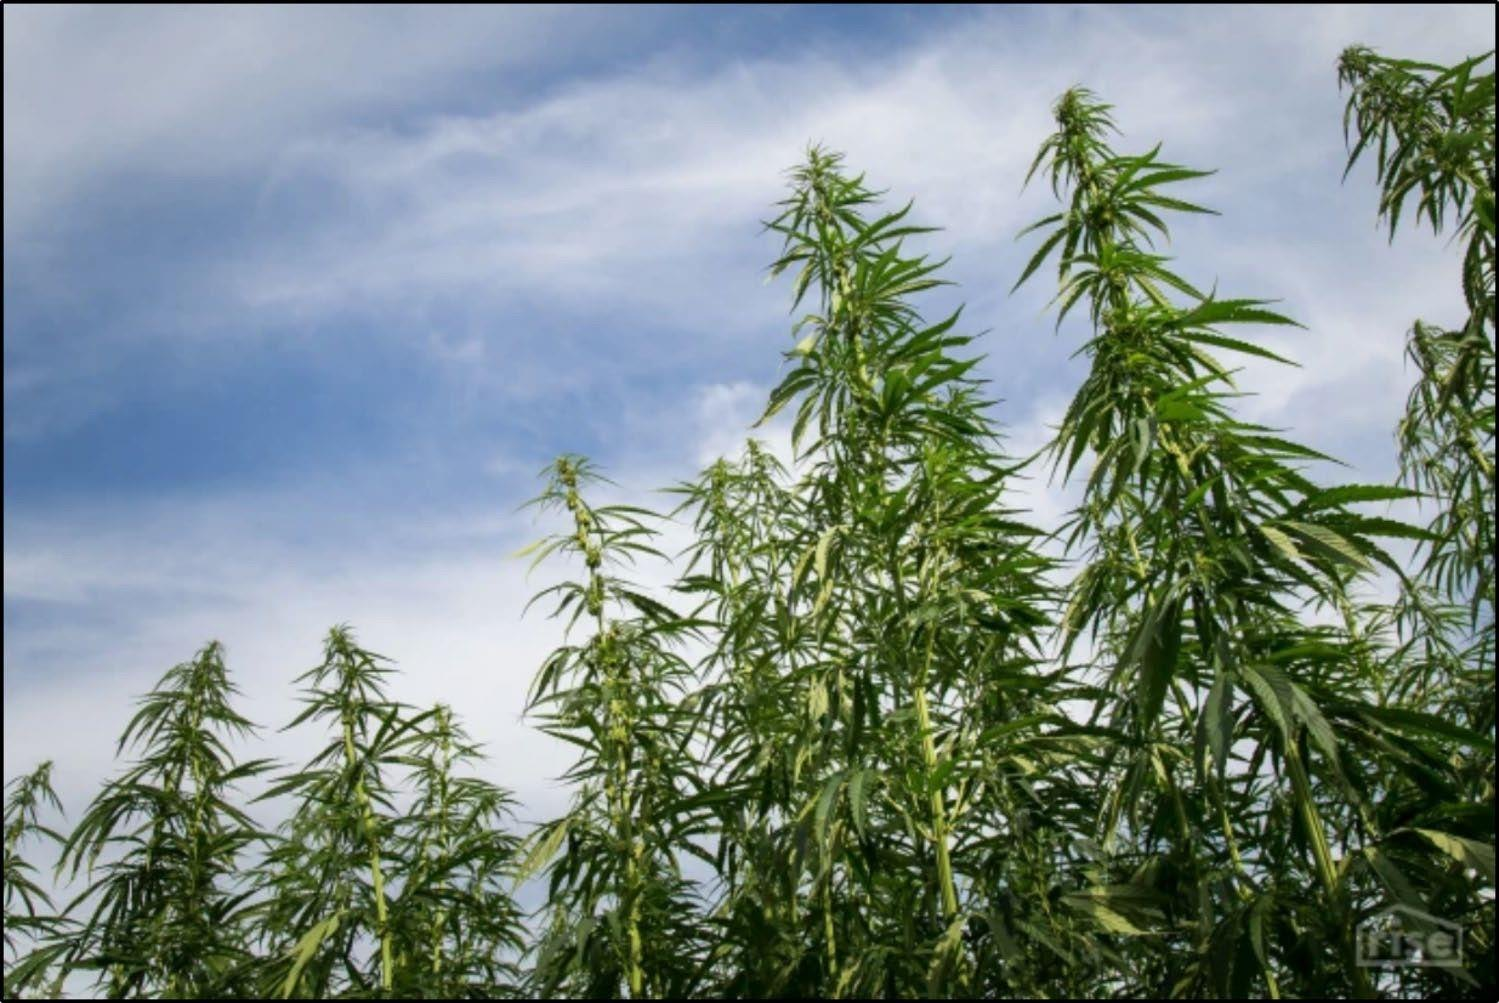
\includegraphics[width=0.72\textwidth]{fig3_1.jpg}
\caption{Industrial hemp}
\end{figure}

The stem structure explains why different portions of hemp have different industrial uses.
Bast fibres occur toward the outside of the cambium and are important in fibre applications,
while the inner woody hurd is the principal particulate component used in hempcrete. The
production process therefore begins with separating the woody core from the other botanical
components.

\section[Hemp Shives]{HEMP SHIVES}
Hemp shives are lightweight, porous and hygroscopic. Their particle size and shape influence
the void structure, binder distribution, density and thermal behaviour of the final composite.
The material is therefore sensitive to raw-material consistency. A change in shive grading can
alter packing and the amount of binder required to achieve a continuous matrix.

\begin{figure}[H]
\centering
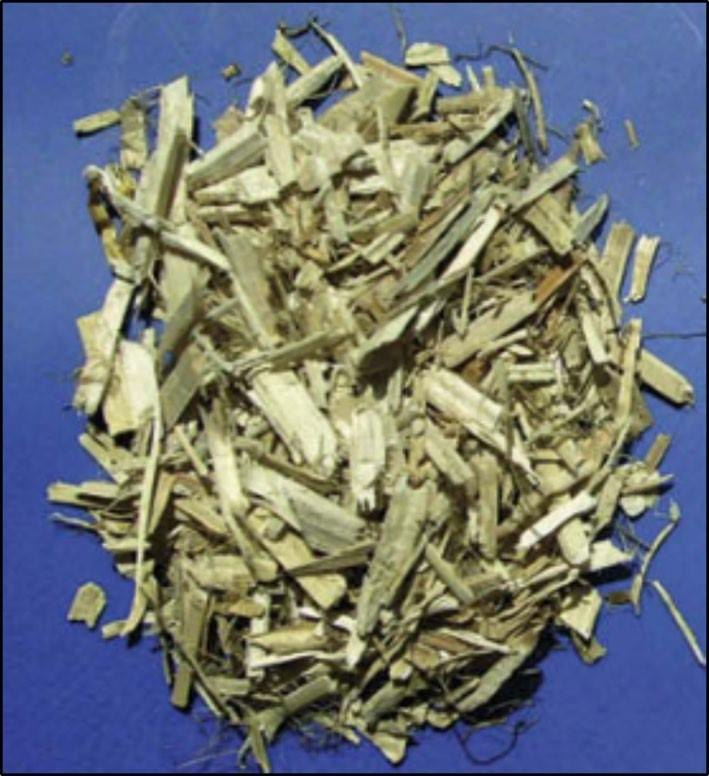
\includegraphics[width=0.55\textwidth]{fig3_2.jpg}
\caption{Hemp shives used as the plant-based aggregate}
\end{figure}

\section[Significance of Hemp Stem Anatomy]{SIGNIFICANCE OF HEMP STEM ANATOMY}
The anatomy of the stem is directly related to the way hemp is processed for construction. The
outer bast region contains fibres that are valuable for textile and composite applications, while
the inner woody hurd is the component that is separated, processed and reduced into shives for
hempcrete. The cambium acts as a transition zone between these regions. Understanding this
structure is therefore useful because the quality and characteristics of the hurd influence the
final composite.

The principal review also notes that hemp can be harvested within a relatively short cropping
cycle of about 90--120 days. After harvesting, the woody core is separated from the other
botanical components. The resulting shives are not an inert aggregate in the conventional
sense. They are porous, hygroscopic and capable of interacting with both water and the
mineral binder. Their internal pore structure contributes to the low density and thermal
behaviour of hempcrete, while their moisture response influences curing and long-term
hygrothermal performance.

The review also discusses hemp harvesting and processing. Hemp can be incorporated into
crop rotation, and the literature reports comparatively modest requirements for fertilization
and plant-protection products. After harvesting, the woody core is separated and processed
into a construction-grade particulate material.

\section[Binder Systems]{BINDER SYSTEMS}
Binders form the mineral matrix around the hemp shives. Lime is the most common binder
category discussed in the literature. Natural hydraulic lime can develop strength through
hydraulic reactions, while hydrated lime gains strength through carbonation. Pozzolanic
additions can alter reaction products and performance. Alternative low-carbon and
geopolymer-type systems have also been investigated.

Binder selection influences density, curing, mechanical strength, thermal conductivity,
acoustic response and environmental impact. This is one reason why published hempcrete
properties cannot be treated as universal constants. A reported strength or conductivity value
must always be interpreted together with the mix composition, density, age and testing
method.

\begin{table}[H]
\centering
\caption{Main constituents of hempcrete}
\begin{tabular}{@{}p{3.3cm}p{4.2cm}p{5.6cm}@{}}
\toprule
\textbf{Constituent} & \textbf{Role} & \textbf{Important variables}\\
\midrule
Hemp shives & Lightweight porous aggregate & Particle size, grading, moisture\\
\addlinespace
Mineral binder & Matrix and bonding & Binder chemistry, content, curing\\
\addlinespace
Water & Workability and reaction & Initial moisture, quantity, drying\\
\addlinespace
Optional additions & Property modification & Pozzolans, water retainers, other modifiers\\
\bottomrule
\end{tabular}
\end{table}

\section[Mix Design]{MIX DESIGN}
Unlike conventional structural concrete, hempcrete has no single universally accepted mix
proportion. The final material depends on the desired density, thermal performance,
construction technique, binder characteristics, water content, hemp-shive properties,
compaction and curing. Increasing density can improve some mechanical properties but can
also increase thermal conductivity. The design problem is therefore a balance between
strength, insulation, moisture behaviour and constructability.

\section[Construction Techniques]{CONSTRUCTION TECHNIQUES}
Common construction approaches include in-situ casting, prefabricated blocks, panels and
spray application. In-situ casting involves mixing hemp shives and binder at the construction
site and placing the material into temporary or permanent formwork around a structural frame.
Prefabricated blocks are manufactured and cured away from the building site. Spray
application can create a continuous layer and is particularly relevant to renovation and
complex surfaces.

\begin{figure}[H]
\centering
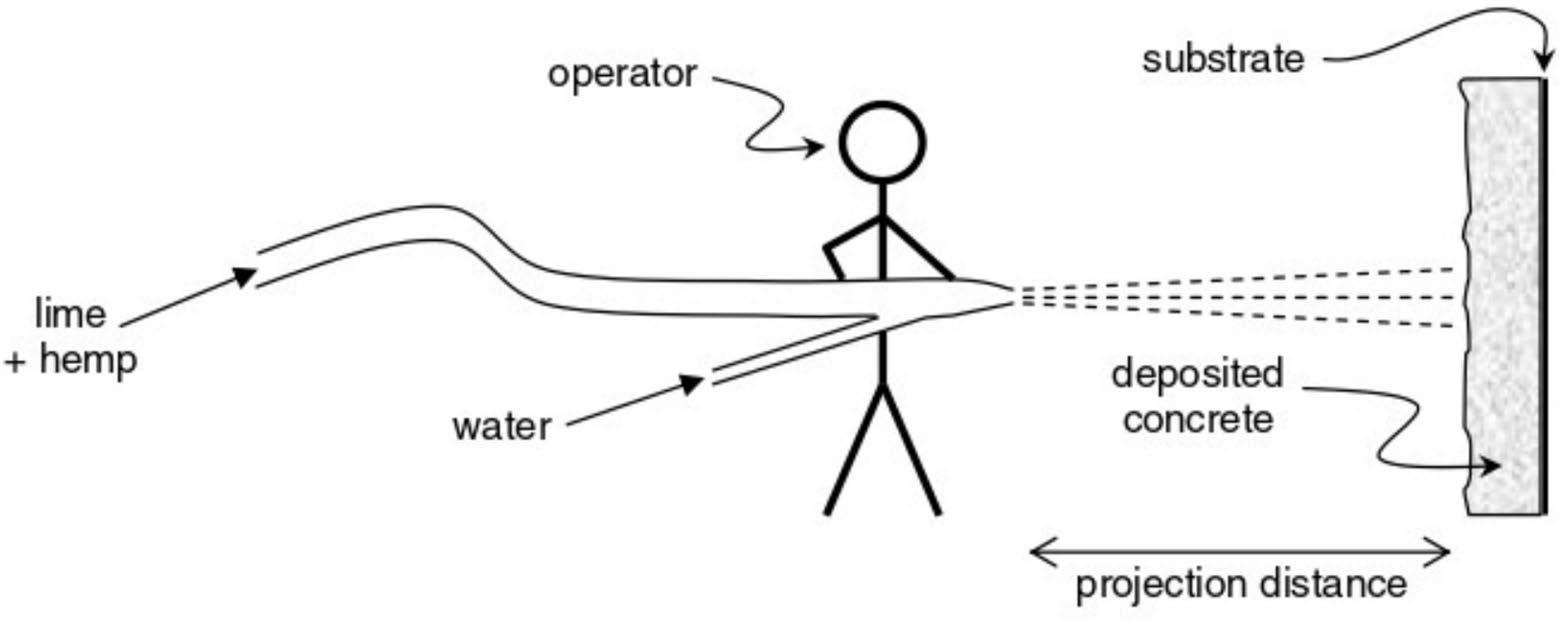
\includegraphics[width=0.78\textwidth]{fig3_3.jpg}
\caption{Spray-applied hempcrete process}
\end{figure}

\begin{figure}[H]
\centering
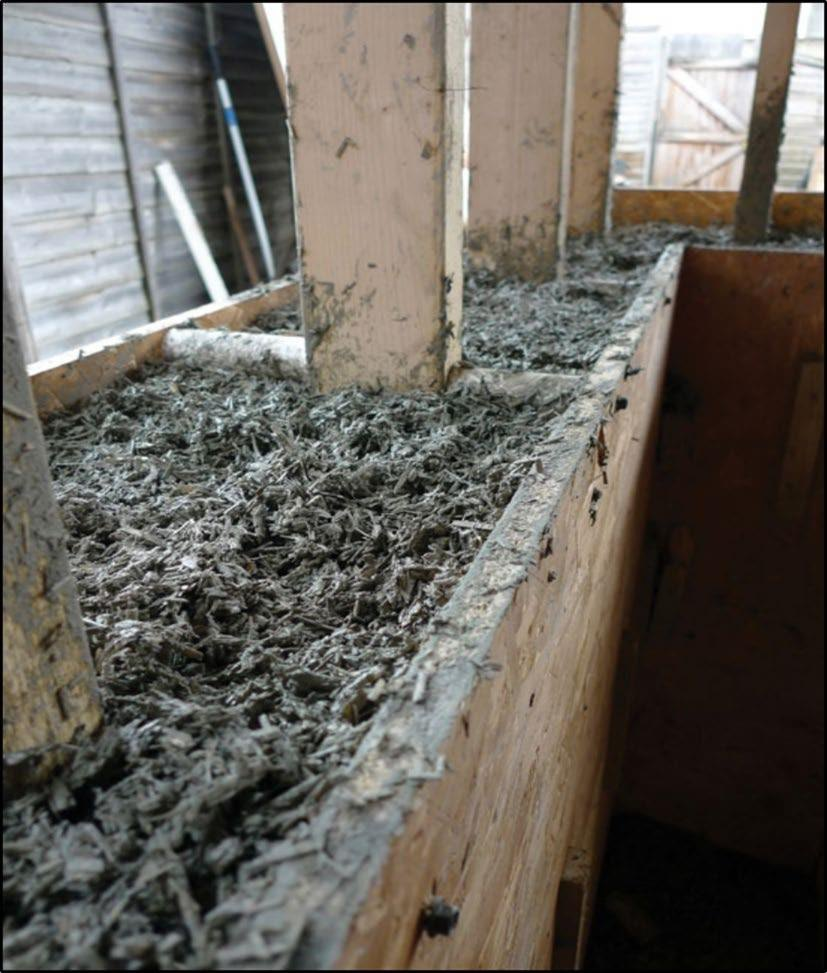
\includegraphics[width=0.60\textwidth]{fig3_4.jpg}
\caption{In-situ hempcrete during wall construction}
\end{figure}

\begin{figure}[H]
\centering
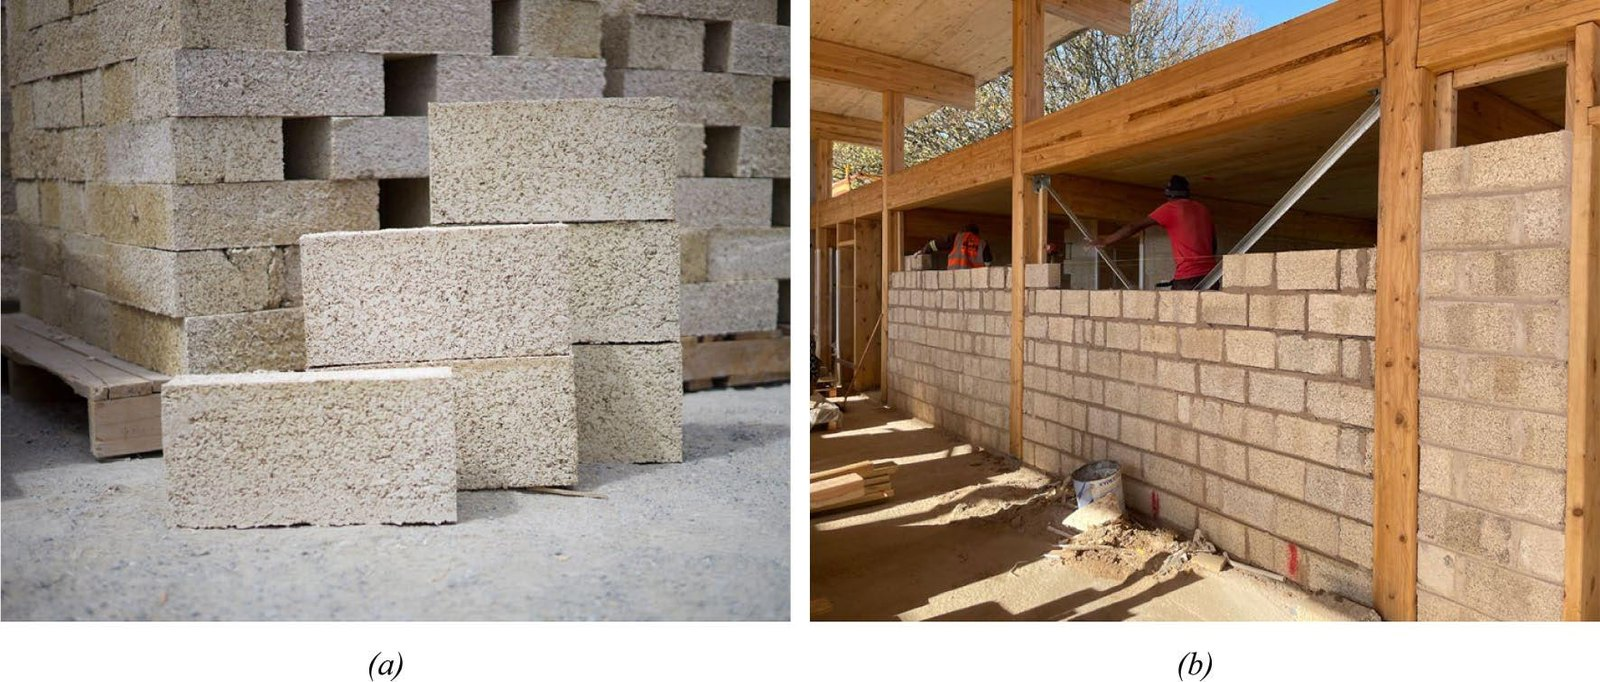
\includegraphics[width=0.88\textwidth]{fig3_5.jpg}
\caption{Prefabricated hempcrete blocks (a) and block-wall construction (b)}
\end{figure}

\section[Fresh-State Properties]{FRESH-STATE PROPERTIES}
Fresh hempcrete is lightweight and porous and is not designed around the high-flow placement
and early compressive strength associated with conventional concrete. Workability depends on
water content, binder type, shive characteristics and mixing sequence. Appropriate tamping or
compaction is required for uniformity, but excessive compaction can reduce porosity and
change thermal performance.

\section[Mechanical Properties]{MECHANICAL PROPERTIES}
Mechanical strength is one of the principal limitations of hempcrete. The porous lightweight
structure produces much lower compressive strength than structural concrete. Consequently,
hempcrete is generally used around a structural frame. The review nevertheless reports that
binder content, hemp-to-binder ratio, density, hemp treatment and binder chemistry can
influence strength. Research is therefore focused on improving strength without losing the
low-density advantages.

\section[Thermal Properties]{THERMAL PROPERTIES}
Thermal insulation is one of hempcrete's strongest engineering advantages. Its porous structure
and low density reduce heat transfer. The principal review reports that many hempcrete
thermal-conductivity values are lower than those of autoclaved aerated concrete at comparable
densities. Moisture, density, binder composition and particle characteristics can all influence
the measured value.

\section[Acoustic Properties]{ACOUSTIC PROPERTIES}
The porous internal structure of hempcrete can absorb sound energy. The principal review
indicates that smaller hemp shives and lime-pozzolanic binders can produce higher sound
absorption in selected studies, while other investigations identify the quantity of hemp shives
as a major determinant. Acoustic performance is therefore dependent on material composition,
density, thickness and assembly configuration.

\section[Moisture and Durability]{MOISTURE AND DURABILITY}
Hempcrete is hygroscopic and can absorb and release water vapour as surrounding humidity
changes. This moisture-buffering behaviour can stabilize indoor relative humidity. However,
the same moisture responsiveness requires appropriate wall detailing. Prolonged liquid-water
exposure, inadequate drying paths, poor interfaces or unsuitable finishes can create durability
problems.

\section[Fire Behaviour]{FIRE BEHAVIOUR}
The principal review reports favourable fire-resistant characteristics in several investigated
hempcrete systems. The mineral binder limits the flammability of the plant component, while
density, binder chemistry, coatings and wall assembly influence the final fire response.
Because fire safety is regulatory, project-specific testing and compliance remain necessary.

\section[Construction Quality and Fire Safety]{CONSTRUCTION QUALITY AND FIRE SAFETY}
Fire performance cannot be considered independently of construction quality. The mineral
binder, hemp content, density, moisture condition, surface finish and wall assembly all
influence how heat and flame interact with the material. A laboratory result for one
formulation should therefore not be transferred directly to another wall system. Openings,
service penetrations, joints and surface coatings can also change the behaviour of the
completed assembly.

For practical construction, the engineer should verify that the specified material reaches the
intended density and that the hemp shives are uniformly distributed. Excessive voids, local
segregation or uncontrolled moisture can produce variations in the finished wall. Drying is
particularly important because hempcrete is normally installed with significant moisture and
requires time to reach its service condition. Temporary weather protection and a suitable
drying path are therefore part of quality control.

\section[Material Compatibility and Interfaces]{MATERIAL COMPATIBILITY AND INTERFACES}
The interface between hempcrete and the structural frame is another important consideration.
Timber, masonry, concrete and steel can all be used in building systems containing hempcrete,
but the interface must account for vapour movement, thermal bridging and chemical
compatibility. The high alkalinity of lime-based binders requires particular attention around
vulnerable steel components. Where direct contact cannot be avoided, corrosion protection or
physical separation should be considered.

\section[Limitations of Current Test Data]{LIMITATIONS OF CURRENT TEST DATA}
Published results vary because researchers use different hemp shives, binders, densities, curing
periods and testing methods. This variation makes direct numerical comparison difficult.
Future standards should therefore define material conditioning, specimen geometry, density
classes and test procedures so that reported values can be compared reliably across studies and
projects.

%=====================================================================
% CHAPTER 4 (Advantages and Disadvantages)
%=====================================================================
\chapter{ADVANTAGES AND DISADVANTAGES}

\section[Advantages of Hempcrete]{ADVANTAGES OF HEMPCRETE}

\textbf{Excellent thermal insulation} -- The porous structure of hempcrete provides good
thermal insulation and helps reduce heat transfer through walls, thereby lowering heating and
cooling requirements.

\textbf{Low environmental impact} -- Hemp is a renewable material that requires relatively
little water and pesticide for cultivation. Hempcrete can also store significant amounts of
CO\textsubscript{2} during its life cycle.

\textbf{Lightweight material} -- Hempcrete has a low density, which reduces the load
transferred to foundations and makes handling and construction easier.

\textbf{Moisture regulation} -- Hempcrete is vapour-permeable and can absorb and release
moisture, helping to regulate indoor relative humidity and reduce condensation.

\textbf{Good acoustic performance} -- Its porous structure provides sound absorption, making
hempcrete useful for improving acoustic comfort in buildings.

\textbf{Fire resistance} -- Studies reviewed in the literature indicate that hempcrete can resist
ignition and produce relatively little smoke under fire exposure.

\textbf{Resistance to insects and mould} -- The alkaline nature of lime-based binders provides
protection against insects, mould and biological deterioration under suitable conditions.

\textbf{Easy application and repair} -- Hempcrete can be used for infilling and renovation, and
its lightweight nature makes construction and repair comparatively convenient.

\section[Disadvantages of Hempcrete]{DISADVANTAGES OF HEMPCRETE}

\textbf{Low compressive strength} -- Hempcrete has much lower compressive strength than
conventional concrete and is therefore generally used as a non-load-bearing material.

\textbf{High water absorption} -- Hempcrete can absorb considerable amounts of water.
Prolonged exposure to moisture without adequate ventilation may create durability problems
such as biological decay and freeze-thaw damage.

\textbf{Long drying time} -- Hempcrete contains moisture during construction and requires
adequate drying before finishes can be applied. High humidity can further delay drying.

\textbf{Shrinkage} -- Shrinkage can occur during drying, and the binder type has a significant
influence on the amount of shrinkage.

\textbf{Requires skilled labour} -- Contractors and workers need knowledge of hempcrete
mixing, placement, compaction and drying requirements. Lack of trained labour can restrict its
wider use.

\textbf{Limited availability} -- Hempcrete is not as widely available as conventional
construction materials, and regulations related to hemp cultivation can affect its availability in
some regions.

\textbf{Lack of standardization} -- Standardized guidelines for hempcrete mix designs,
applications and performance are still needed to ensure consistent quality.

%=====================================================================
% CHAPTER 5 (Results and Discussion)
%=====================================================================
\chapter{RESULTS AND DISCUSSION}

\section[Compatibility with Timber]{COMPATIBILITY WITH TIMBER}
Hempcrete is frequently associated with timber-frame construction because both materials can
be incorporated into vapour-permeable wall assemblies. The review notes that hempcrete can
help provide a protective environment for timber. However, exposure conditions and external
cladding systems still require appropriate detailing.

\begin{figure}[H]
\centering
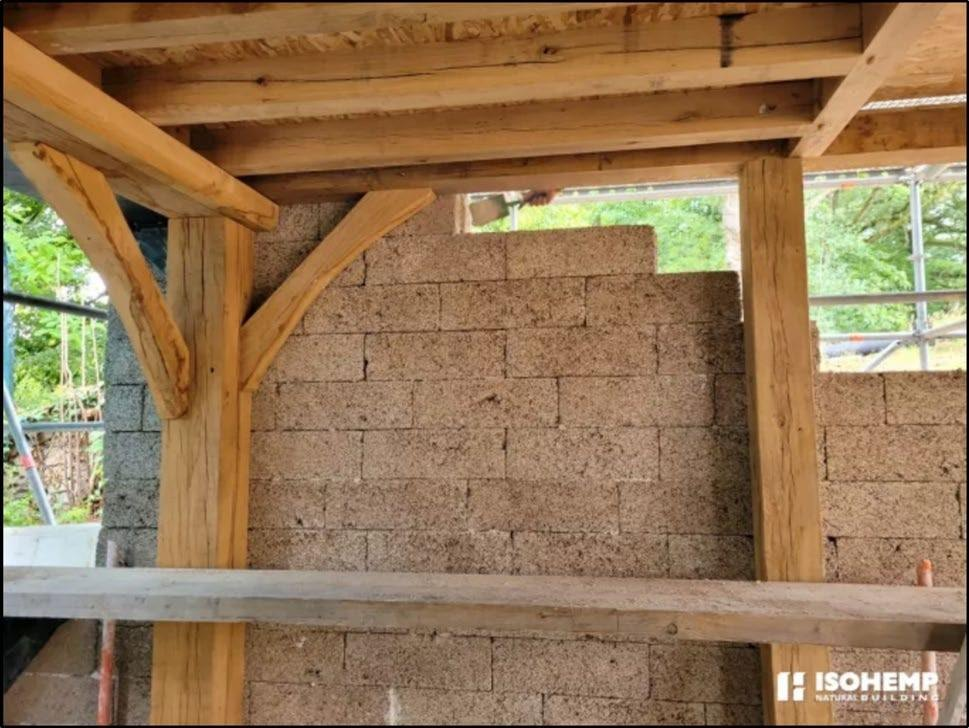
\includegraphics[width=0.62\textwidth]{fig4_1.jpg}
\caption{Hempcrete blocks utilised in a timber post-and-beam structure}
\end{figure}

\section[Compatibility with Masonry and Steel]{COMPATIBILITY WITH MASONRY AND STEEL}
Hempcrete can be cast against masonry walls as an insulating material. Existing gypsum
plasters or cement renders may need to be removed where they are incompatible with a
vapour-permeable lime-hemp assembly. Steel requires additional care because the alkaline
environment associated with lime binders can create corrosion concerns. The review
recommends separating steel frames from the hempcrete where practical, or protecting steel
components with appropriate anti-corrosion measures.

\begin{figure}[H]
\centering
\begin{minipage}[b]{0.48\textwidth}\centering
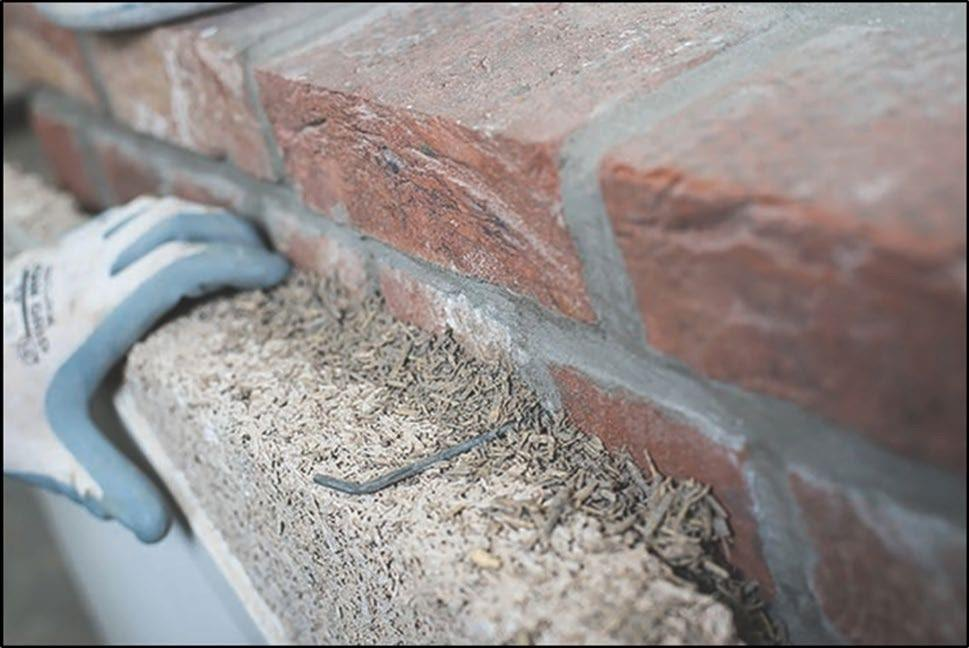
\includegraphics[width=\textwidth]{fig4_2a.jpg}\\[2pt]{\small (a)}
\end{minipage}\hfill
\begin{minipage}[b]{0.40\textwidth}\centering
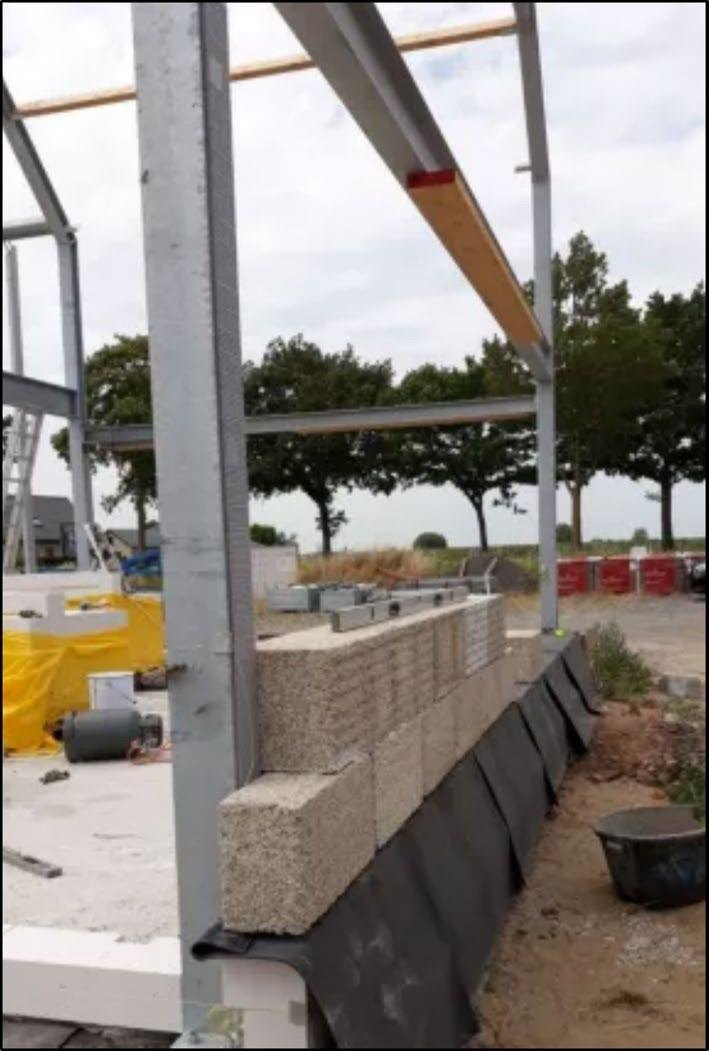
\includegraphics[width=\textwidth]{fig4_2b.jpg}\\[2pt]{\small (b)}
\end{minipage}
\caption{Hempcrete cast against masonry (a) and used with a metal structural system (b)}
\end{figure}

\section[Real-World Application: Hemp Hotel]{REAL-WORLD APPLICATION: HEMP HOTEL}
The Hemp Hotel in Cape Town, South Africa, was completed in June 2023 and opened to the
public in August 2023. The 12-storey building incorporates hempcrete as an infill material
while concrete and cement provide the structural framework. The project is significant because
it demonstrates the use of hemp-based material within a multi-storey urban building rather
than limiting the technology to small low-rise structures.

\begin{figure}[H]
\centering
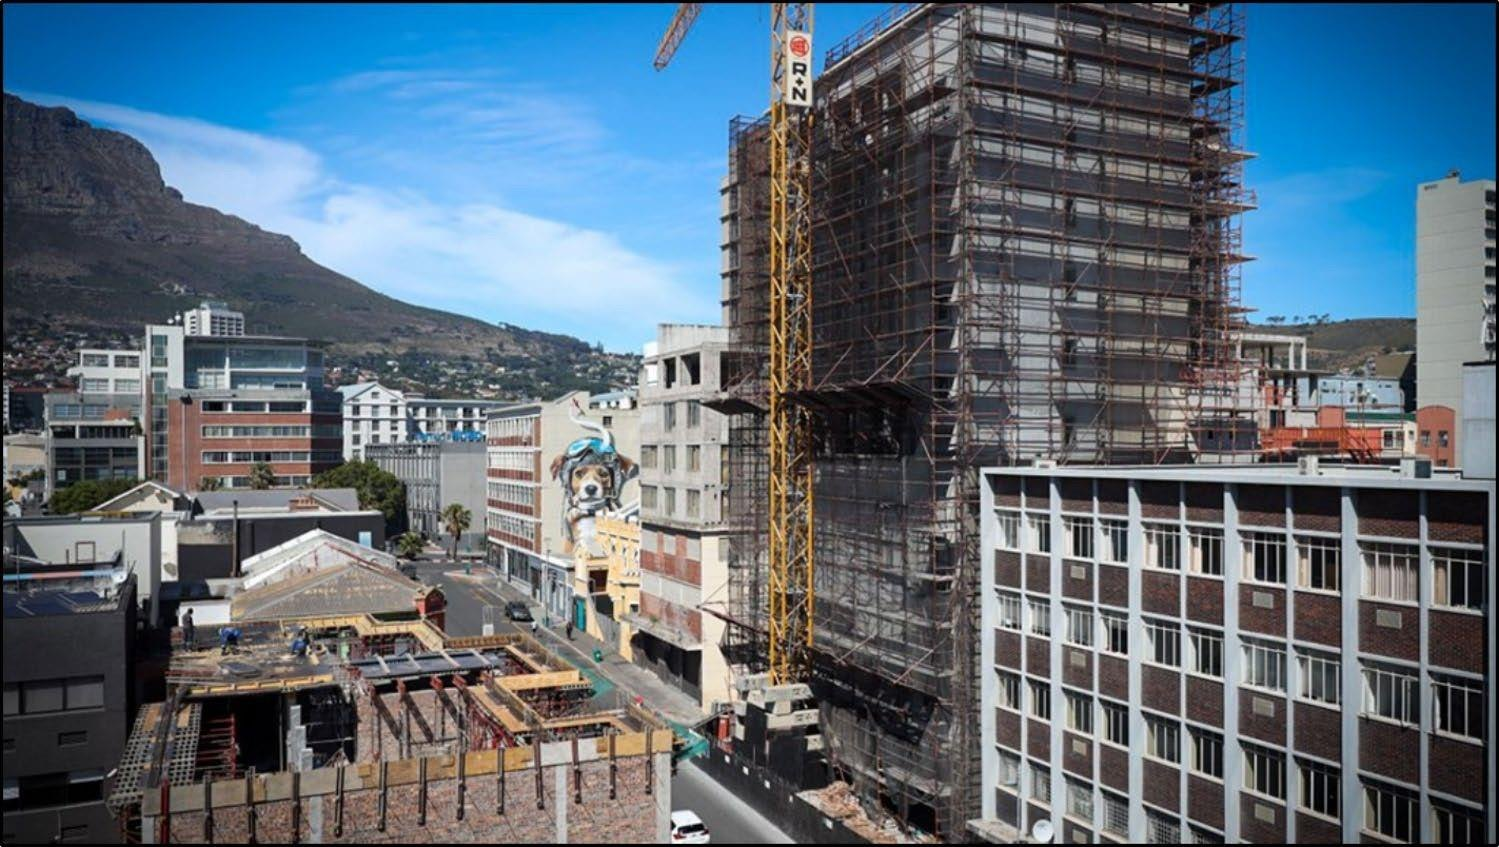
\includegraphics[width=0.72\textwidth]{fig4_3.jpg}
\caption{Hemp Hotel under construction, Cape Town}
\end{figure}

\begin{figure}[H]
\centering
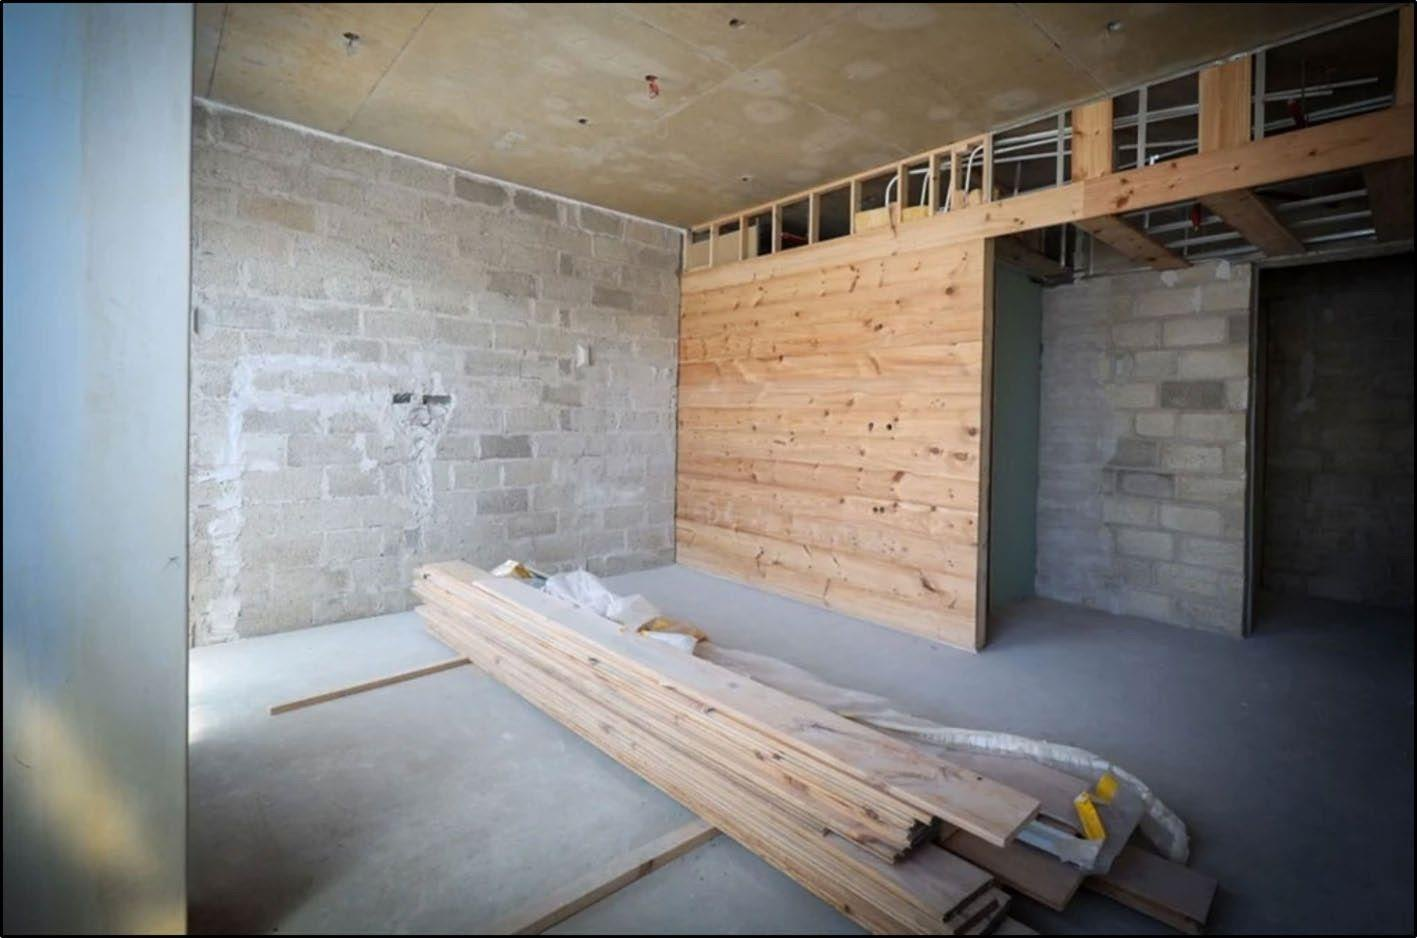
\includegraphics[width=0.72\textwidth]{fig4_4.jpg}
\caption{Interior construction of the Hemp Hotel}
\end{figure}

\section[Adnams Brewers Distribution Centre]{REAL-WORLD APPLICATION: ADNAMS BREWERS DISTRIBUTION CENTRE}
The Adnams Brewers Distribution Centre in Suffolk, United Kingdom, represents a larger
commercial application. The project used locally sourced hemp shives and lime for
approximately 1000~m\textsuperscript{3} of in-situ cast hempcrete together with roughly
100,000 hempcrete blocks. The project demonstrates that hempcrete can be deployed at a scale
considerably beyond laboratory specimens.

\begin{figure}[H]
\centering
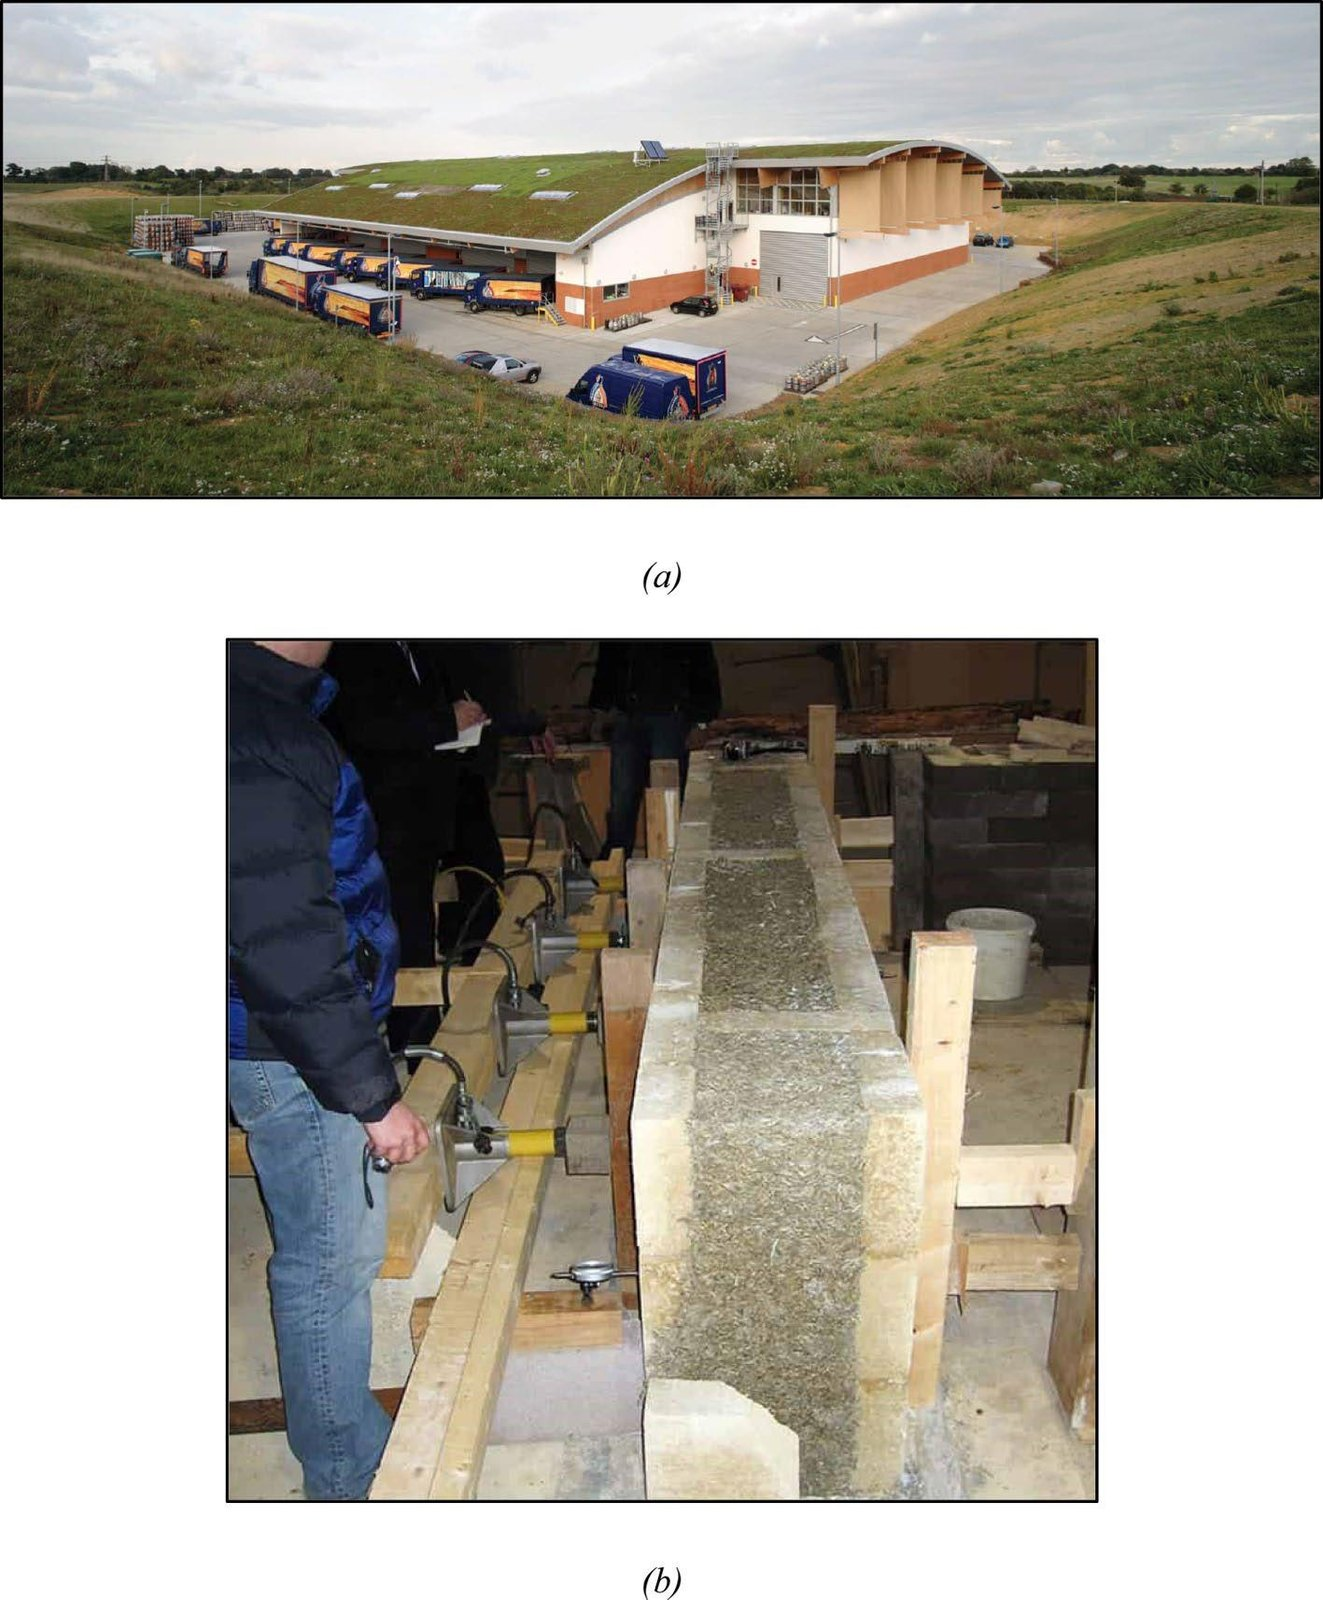
\includegraphics[width=0.66\textwidth]{fig4_5.jpg}
\caption{Adnams Brewers Distribution Centre: exterior (a) and in-situ casting (b)}
\end{figure}

\section[Pierre Chevet Sports Hall]{PIERRE CHEVET SPORTS HALL}
The Pierre Chevet Sports Hall in France was constructed in 2021 using hempcrete blocks and
wood. The project is described in the principal review as France's first exclusive commercial
hempcrete structure. Its significance lies in demonstrating how hempcrete blocks can form a
major component of a commercial building system.

\begin{figure}[H]
\centering
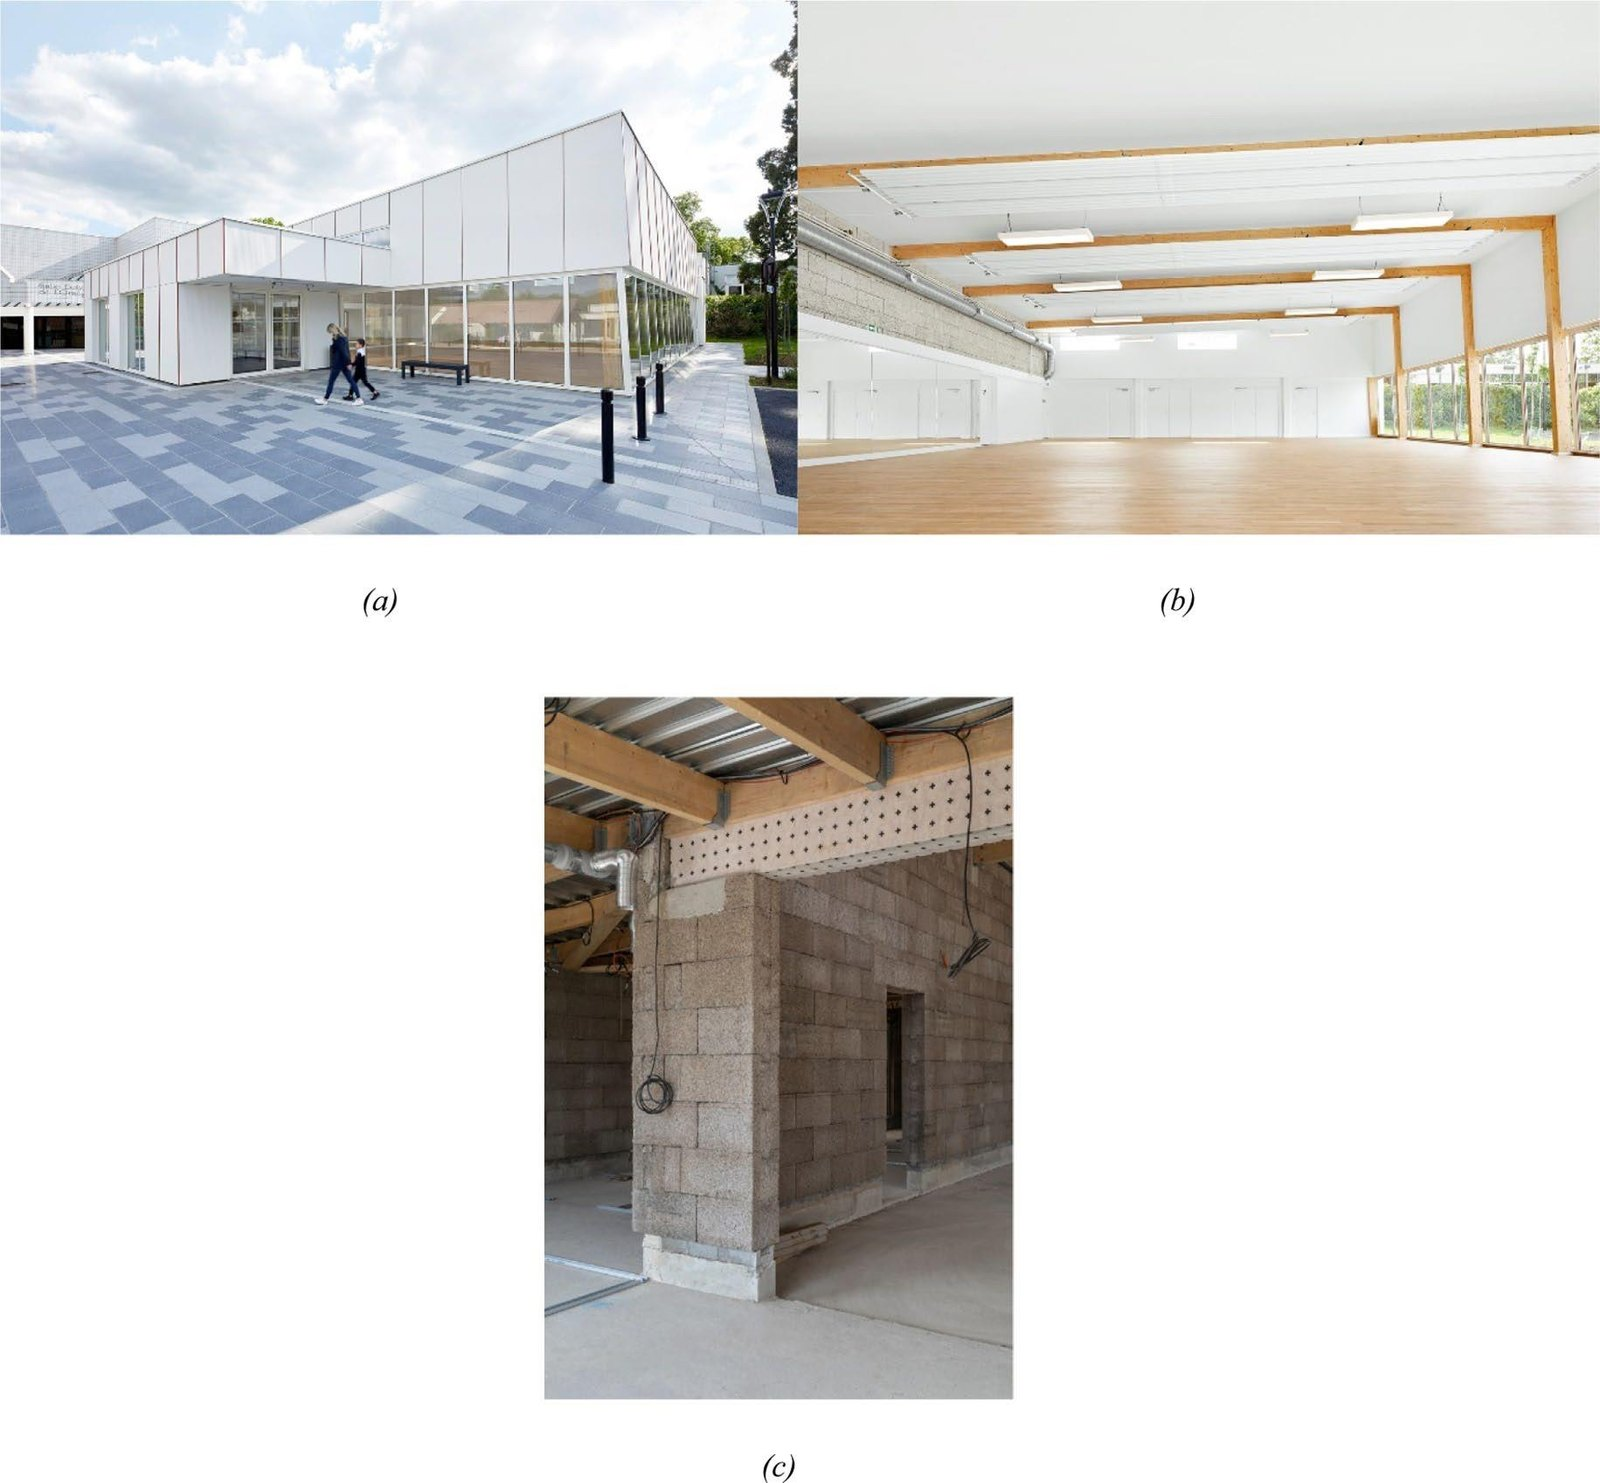
\includegraphics[width=0.78\textwidth]{fig4_6.jpg}
\caption{Pierre Chevet Sports Hall, France}
\end{figure}

\section[Hygrothermal Performance in Different Climates]{HYGROTHERMAL PERFORMANCE IN DIFFERENT CLIMATES}
The review examines studies in France, Italy and Canada. In a hempcrete building in southwest
France, reported indoor temperatures remained comparatively stable despite seasonal outdoor
variations. A controlled climatic-chamber investigation in southern Italy also showed the
ability of hempcrete walls to moderate internal humidity. A study comparing hempcrete and
conventional wood-frame buildings in Vancouver and Toronto found that hempcrete reduced
annual overheating hours in both climates.

\begin{figure}[H]
\centering
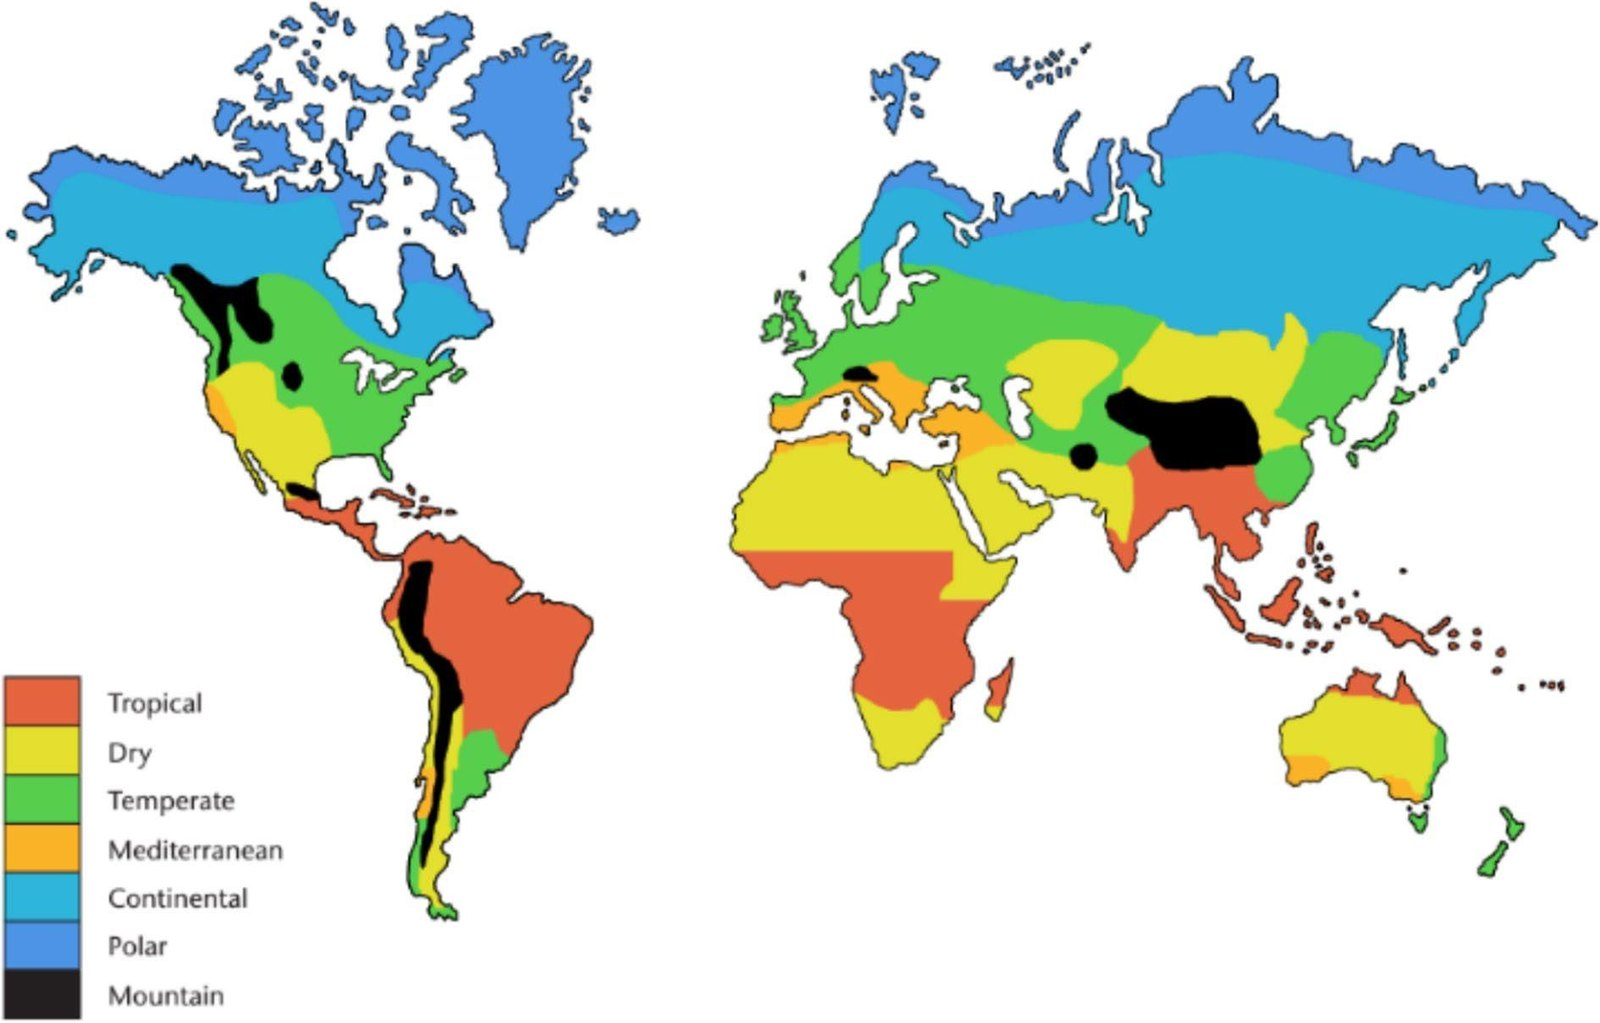
\includegraphics[width=0.86\textwidth]{fig4_7.jpg}
\caption{Climate zones represented in the reviewed performance studies}
\end{figure}

The review reports that hempcrete reduced overheating hours by 21.7\% in Vancouver and
26.9\% in Toronto. These findings indicate that hempcrete can moderate indoor temperature
peaks under the investigated conditions, potentially improving occupant comfort and reducing
reliance on air-conditioning systems.

\begin{figure}[H]
\centering
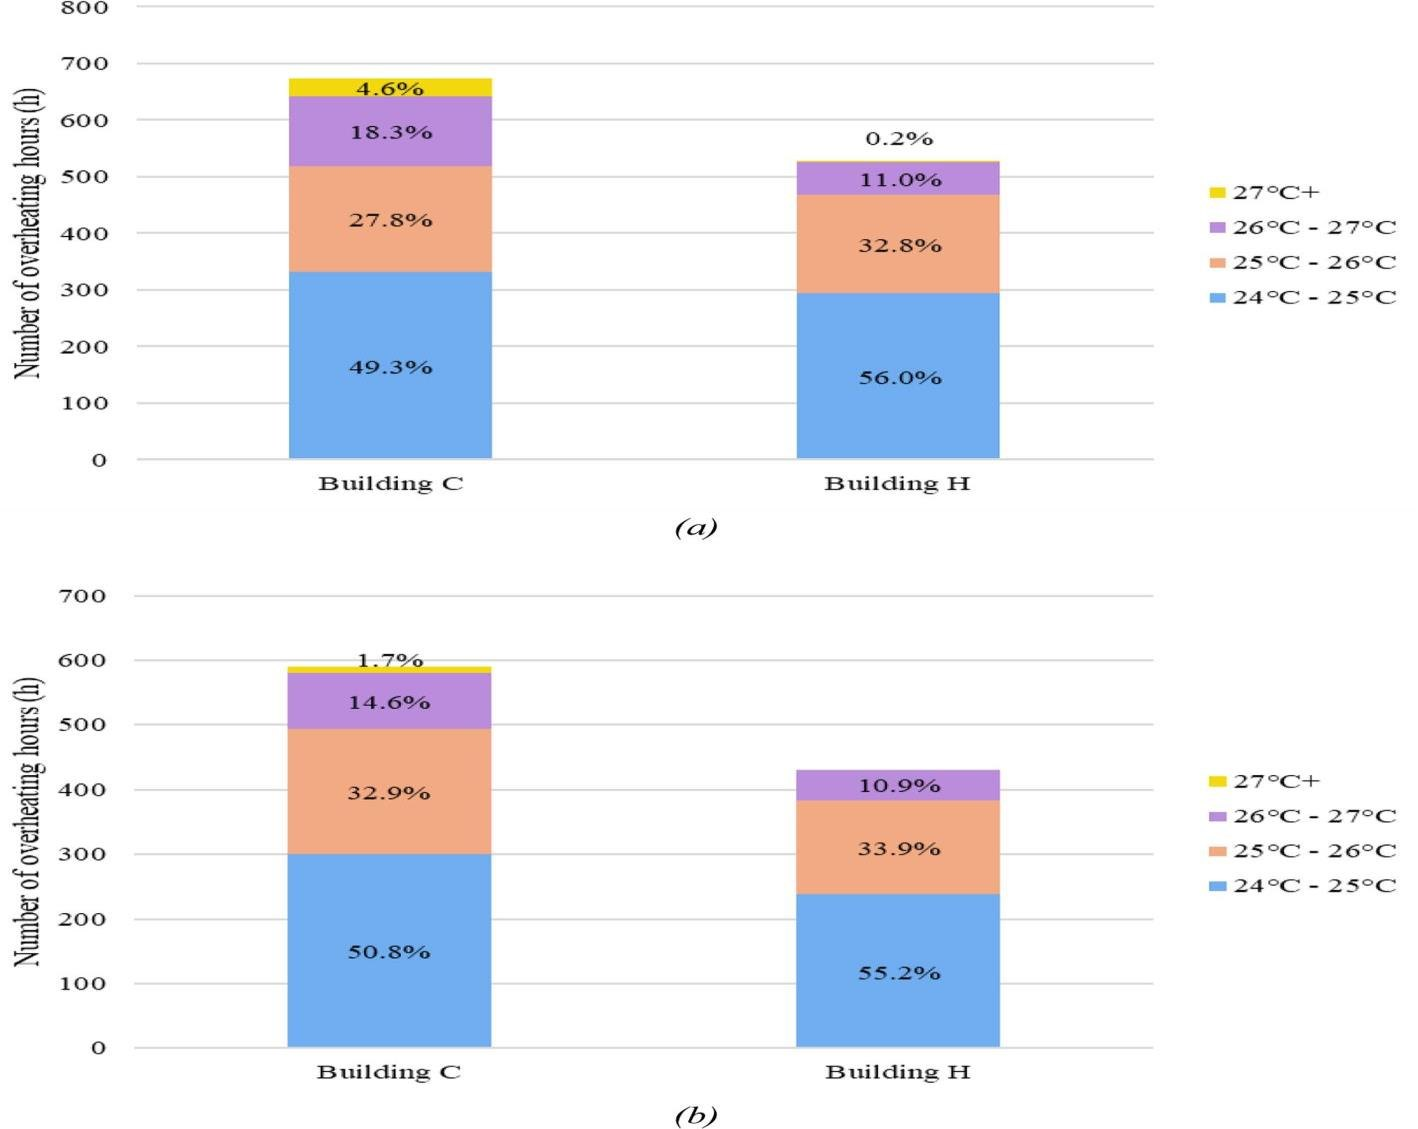
\includegraphics[width=0.70\textwidth]{fig4_8.jpg}
\caption{Annual overheating hours reported for the compared buildings}
\end{figure}

\section[Environmental Performance]{ENVIRONMENTAL PERFORMANCE}
The environmental performance of hempcrete is closely connected to carbon storage. Hemp
absorbs carbon dioxide during growth, and carbon remains embodied in the plant material after
it becomes part of a building component. The lime binder can also absorb carbon dioxide
during carbonation. Several life-cycle studies reviewed by Steyn et al. identify hempcrete as
having potential to act as a carbon sink, but the magnitude of the benefit depends on the
system boundary and assumptions.

\section[Life-Cycle Assessment]{LIFE-CYCLE ASSESSMENT}
Life-cycle assessment must include cultivation, agricultural operations, processing, binder
production, transport, construction, service life and end-of-life. The review notes that
raw-material production, transportation distance and binder composition can strongly influence
the environmental result. It is therefore inappropriate to describe hempcrete as automatically
carbon-negative without defining the life-cycle boundary.

\section[Economic Considerations]{ECONOMIC CONSIDERATIONS}
Cost depends on local hemp availability, processing infrastructure, binder supply, labour,
equipment and construction familiarity. Some projects may have higher initial construction
costs because specialist training or drying periods are required. However, the review also
describes cases where improved indoor environmental control and lower operational energy can
provide long-term economic benefits.

\section[Science Museum Group Storage Facility]{SCIENCE MUSEUM GROUP STORAGE FACILITY}
The Science Museum Group storage facility in Wiltshire, United Kingdom, is another useful
demonstration of hempcrete at building scale. The project incorporated precast hempcrete
panels within a three-storey storage facility containing approximately 930~m\textsuperscript{2}
of storage space. The facility was designed to provide a stable and controlled indoor
environment for archival collections, making hygrothermal performance particularly important.

The principal review reports that the facility required a longer drying period than initially
anticipated. However, monitoring indicated that the hygrothermal behaviour of the hempcrete
helped maintain suitable conditions for the stored collections during the stabilization phase.
The review also cites a construction cost approximately 10\% greater than conventional
museum storage facilities, while operational costs were reported to be reduced by more than
50\% compared with similarly sized climate-controlled spaces.

\section[Interpretation of Real-World Applications]{INTERPRETATION OF REAL-WORLD APPLICATIONS}
The case studies demonstrate that hempcrete is not limited to experimental wall specimens. Its
applications range from timber-frame houses and masonry retrofits to commercial distribution
centres, sports halls, museum storage and multi-storey buildings. The common feature is that
the structural and envelope roles are clearly coordinated. Hempcrete provides insulation,
moisture regulation and other envelope functions while a suitable frame or supporting system
carries the primary structural loads.

These projects also show why project-specific design is essential. Local climate, supply chains,
drying conditions, labour skills and building regulations affect the feasibility of hempcrete. A
successful demonstration in one country cannot simply be copied without considering the
environmental and construction conditions of another region. For civil engineers, the correct
approach is therefore to evaluate hempcrete as part of an integrated building system.

%=====================================================================
% CHAPTER 6
%=====================================================================
\chapter{CONCLUSION}
\section[Conclusion]{CONCLUSION}
\begin{itemize}[label=\textbullet,leftmargin=2.4em,itemsep=6pt,topsep=2pt,parsep=0pt]
\item Hempcrete is a promising and sustainable building material that combines low density, thermal insulation, acoustic performance and moisture buffering.
\item It offers biogenic carbon storage because hemp absorbs carbon dioxide while growing.
\item Its performance depends on hemp-shive characteristics, binder chemistry, mix proportion, density and curing conditions.
\item Its mechanical strength is low, so it is suited to non-load-bearing infill and insulation within a structural frame.
\item Real-world projects show that it can be integrated with timber, masonry, steel and concrete systems.
\item Moisture management, fire protection and quality control are essential.
\item Overall, hempcrete is not a replacement for concrete but an effective low-carbon envelope material.
\end{itemize}
\newpage
\section[Future Scope]{FUTURE SCOPE}
Future research on hempcrete should focus on standardized mix designs and test methods, and on
improving strength and ductility through optimized binders, additives and reinforcement.
Long-term durability studies under realistic humidity cycles and whole-assembly fire studies are
needed, together with life-cycle assessments using consistent system boundaries and economic
studies of local supply chains and prefabricated components. Research on reuse and recycling,
along with standardized design methods, specifications and regulations, will support the wider
adoption of hempcrete as a reliable engineering material.

Fire-safety studies should evaluate complete wall assemblies rather than isolated specimens,
considering density, binder chemistry, coatings, joints and service penetrations. Long-term
monitoring of completed hempcrete buildings in different climates would provide valuable data
on drying behaviour, moisture performance and durability in service, and training programmes
for designers and contractors, together with reliable local supply chains for hemp shives and
binders, would help reduce construction errors and cost.

%=====================================================================
% REFERENCES
%=====================================================================
\newpage
\frontheading{REFERENCES}
\addcontentsline{toc}{chapter}{REFERENCES}

\begingroup\hyphenpenalty=10000 \exhyphenpenalty=10000
\begin{enumerate}[label=\roman*.,leftmargin=2.4em,itemsep=10pt]
\item \textbf{S. Elfordy et al.,} \textit{``Mechanical and thermal properties of lime and hemp concrete (hempcrete) manufactured by a projection process,''} Construction and Building Materials, vol. 22, issue 10, 2024, pp.~2116--23.

\item \textbf{R. Haik et al.,} \textit{``Lime hempcrete composites based on unfired binders: a review,''} Circular Economy and Sustainability, vol. 5, issue 3, 2025, pp.~2609--19.

\item \textbf{T. Jami et al.,} \textit{``A review of the properties of hemp concrete for green building applications,''} Journal of Cleaner Production, vol. 239, art. no. 117852, 2025.

\item \textbf{S. G. Nair et al.,} \textit{``Low-carbon calcined clay-based binders for sustainable hempcrete,''} Materials and Structures, vol. 58, issue 6, art. no. 204, 2025.

\item \textbf{K. Steyn et al.,} \textit{``A comprehensive review of hempcrete as a sustainable building material,''} Innovative Infrastructure Solutions, vol. 10, issue 3, art. no. 97, 2025.
\end{enumerate}
\endgroup

\end{document}
